\documentclass[runningheads]{llncs}
\usepackage{amsmath}
\usepackage{amsfonts}
\usepackage{mathtools}
\usepackage{color}
\usepackage{graphicx}
\usepackage{listings}
\usepackage{wasysym}
\usepackage[lighttt]{lmodern}
\usepackage{siunitx}
\usepackage{hyperref}
% If you use the hyperref package, please uncomment the following line
% to display URLs in blue roman font according to Springer's eBook style:
 \renewcommand\UrlFont{\color{blue}\rmfamily}

\newcommand\Dist{\mathit{Dist}}
\newcommand\ctrl{\mathit{ctrl}}
\newcommand\prnt{\mathit{prnt}}
\newcommand\link{\mathit{link}}
\newcommand\ar{\mathit{ar}}
\newcommand\id{\mathsf{id}}
\newcommand\Id{\mathsf{Id}}

\providecommand\longrightarrowRHD{\relbar\joinrel\relbar\joinrel\mathrel\RHD}
\providecommand\longrightarrowrhd{\relbar\joinrel\relbar\joinrel\mathrel\rhd}
\providecommand\longrightdoublearrowRHD{\mathrel\LHD\joinrel\relbar\joinrel\relbar\joinrel\mathrel\RHD}

\makeatletter
\providecommand*\xrightarrowRHD[2][]{\ext@arrow 0055{\arrowfill@\relbar\relbar\longrightarrowRHD}{#1}{#2}}
\providecommand*\xrightarrowrhd[2][]{\ext@arrow 0055{\arrowfill@\relbar\relbar\longrightarrowrhd}{#1}{#2}}
\makeatother

\lstdefinelanguage{Big}{
  basicstyle=\ttfamily,
  sensitive=true,
  morekeywords={fun, brs, end, sbrs, pbrs, nbrs, begin, init, atomic, preds,
    rules, action, big, ctrl, float, int, react},
  comment=[l]{\#}
}

\ttfamily
\DeclareFontShape{OT1}{lmtt}{m}{it}
     {<->sub*lmtt/m/sl}{}

\begin{document}
\title{Nondeterministic Bigraphical Reactive Systems for Markov Decision
  Processes\thanks{Supported by organization x.}}
\titlerunning{Nondeterministic BRSs for MDPs}
\author{Paulius Dilkas}
\authorrunning{P. Dilkas}
\institute{University of Glasgow, Glasgow, UK}
\maketitle

\begin{abstract}
  In this paper we introduce two extensions of bigraphical reactive systems
  (BRSs) to handle probabilistic and nondeterministic behaviour, allowing BRSs
  to be used in discrete-time Markov chain and Markov decision process (MDP)
  generation. We extend the implementation of an open-source tool for BRSs
  BigraphER with new syntax for MDP actions and rewards, better visualisation
  capabilities, and data export options. Furthermore, we introduce a new
  front-end for working with BRSs based on Jupyter notebooks, allowing the user
  to quickly visualise bigraphs and reaction rules, simulate execution, or
  produce a complete transition system, all within the notebook interface.
  Finally, we demonstrate the modelling capabilities of the new system with a
  case study on the movement and behaviour of autonomous agents, exploring ideas
  such as collecting objects, tracking visited locations, hierarchies of spaces,
  and uncertainty in the topology of space.

\keywords{Bigraphs \and Bigraphical reactive systems \and Probabilistic
  semantics \and Markov decision process \and Spatial models.}
\end{abstract}

\section{Introduction}

% TODO: introduction
%Bigraphical reactive systems (BRS) \cite{DBLP:books/daglib/0022395} are a
%universal formalism for modelling interacting systems that evolve in time and
%space.

\subsection{Markov Decision Processes}

\begin{definition}[Markov decision process] \label{mdp}
  For any finite set $X$, let $\Dist(X)$ denote the set of discrete probability
  distributions over $X$. A \emph{Markov Decision Process} is a tuple $ (S,
  \overline{s}, A, P, L)$, where: $S$ is a finite set of states and
  $\overline{s} \in S$ is the initial state; $A$ is a finite set of
  \emph{actions}; $P : S \times A \to \Dist(S)$ is a (partial) probabilistic
  transition function, mapping state-action pairs to probability distributions
  over $S$; $L : S \to 2^P$ is a labelling with atomic propositions.
\end{definition}

\begin{definition}[reward structure]
  A \emph{reward structure} for an MDP $(S, \overline{s}, A, P, L)$ is a pair
  $(\rho, \iota)$, where $\rho : S \to \mathbb{R}$ is the \emph{state reward
    function}, and $\iota : S \times A \to \mathbb{R}$ is the \emph{transition
    reward function}.
\end{definition}

\subsection{Bigraphs}

We begin by introducing some notation used in the definitions. Natural numbers
are sometimes interpreted as finite ordinals, i.e., $m = \{ 0, \dots, m - 1 \}$.
We write $S \uplus T$ to indicate the union of sets known or assumed to be
disjoint. For two functions $f$ and $g$ with disjoint domains $S$ and $T$ we
write $f \uplus g$ for the function with domain $S \uplus T$ such that $(f
\uplus g)|_S = f$ and $(f \uplus g)|_T = g$. The identity function on the set
$S$ is written as $\Id_S$. Given a binary relation $\mathit{rel} \subseteq A
\times B$, we denote the domain restriction of $\mathit{rel}$ over $S \subseteq
A$ by $S \lhd \mathit{rel}$. Similarly, we write $\mathit{rel} \rhd S$ for the
range restriction of $\mathit{rel}$ over $S \subseteq B$. We also denote the
transitive closure of $\mathit{rel}$ by $\mathit{rel}^+$. In defining bigraphs
we assume that names, node identifiers, edge identifiers, and controls are drawn
from four infinite pairwise disjoint sets, respectively $\mathcal{X},
\mathcal{V}, \mathcal{E}$, and $\mathcal{K}$.

\begin{figure}
  \centering
  \includegraphics{models/example_bigraph/foo_lhs.pdf}
  \caption{An example bigraph.}
  \label{example_bigraph}
\end{figure}

Informally, a bigraph can be thought of as a graph, where a node can be inside
another node\footnote{To be specific, in this paper we extend the ideas behind
  \emph{bigraphs with sharing}
  \cite{DBLP:phd/ethos/Sevegnani12,dblp:journals/tcs/sevegnanic15}, where a node
  can be contained in the intersection of several other nodes.}. However, the
pictures tend to become much clearer if we instead visualise the nesting
relations between nodes as just a different type of edges. Consider the bigraph
in Fig.~\ref{example_bigraph}. The white ellipses are the \emph{nodes}. Each
node has a type, called \emph{control}, and denoted here by the labels
$\mathsf{A}, \mathsf{B}$, and $\mathsf{C}$. The green edges are actually
hyperedges (can connect any positive number of nodes), and are called
\emph{links}. In this example they are given names $\mathsf{x}, \mathsf{y}$, and
$\mathsf{e}$. Each node has an ordered list of \emph{ports} (not pictured in the
diagram) that can be thought of as sockets for links. Nodes of the same control
have the same number of ports. The number of ports a node of control
$\mathsf{K}$ can have is called the \emph{arity} of $\mathsf{K}$ and is denoted
by $\ar(\mathsf{K})$. The two white dashed rectangles represent \emph{regions},
and in this representation are the parents to any otherwise parentless nodes.
Grey dashed rectangles are called \emph{sites}, and encode parts of the model
that have been abstracted away. Nodes, sites, and regions are also known as
\emph{places}. The directed black arrows between places show the containment
relations, e.g., the $\mathsf{A}$ node has two children (inner nodes):
$\mathsf{B}$ and the only site in this bigraph, labelled by the number $0$.

Another, more formal way to think about a bigraph is as a pair of graphs: one
for describing the placement of nodes, and one for the links between them. This
is the approach that will be featured in our formal definitions. We also focus
on \emph{concrete} bigraphs, where nodes and links have distinct identifiers.

\begin{definition}[concrete place graph with sharing]
  A \emph{concrete place graph with sharing}
  \[ F = (V_F, \ctrl_F, \prnt_F) : m \to n \]
  is a triple having an inner interface $m$ and an outer interface $n$. These
  index the sites and regions of the place graph, respectively. $F$ has a finite
  set $V_F \subset \mathcal{V}$ of nodes, a control map $\ctrl_F : V_F \to
  \mathcal{K}$, and a \emph{parent relation}
  \[ \prnt_F \subseteq (m \uplus V_F) \times (V_F \uplus n) \]
  that is acyclic, i.e., $(v, v) \not\in \prnt_F^+$ for any $v \in V_F$.
\end{definition}

We define several operations on place graphs that will be used later.

\begin{definition}[composition for place graphs with sharing]
  If $F : k \to m$ and $G : m \to n$ are two concrete place graphs with sharing
  with $V_F \cap V_G = \emptyset$, their composite
  \[ G \circ F = (V, \ctrl, \prnt) : k \to n \]
  has nodes $V \coloneqq V_F \uplus V_G$ and a control map $\ctrl \coloneqq
  \ctrl_F \uplus \ctrl_G$. Its parent relation $\prnt \subseteq (k \uplus V)
  \times (V \uplus n)$ is given by:
  \[ \prnt \coloneqq \prnt_G^\lhd \uplus \prnt_\circ \uplus \prnt_F^\rhd, \]
  where
  \begin{align*}
    \prnt_F^\rhd &= \prnt_F \rhd V_F, \\
    \prnt_G^\lhd &= V_G \lhd \prnt_G, \\
    \prnt_\circ &= (m \lhd \prnt_G) \circ (\prnt_F \rhd m).
  \end{align*}
\end{definition}

\begin{definition}[tensor product for place graphs]
  If 
  \[ G_0 = (V_{G_0}, \ctrl_{G_0}, \prnt_{G_0}) : m_0 \to n_0 \]
  and
  \[ G_1 = (V_{G_1}, \ctrl_{G_1}, \prnt_{G_1}) : m_1 \to n_1 \]
  are two concrete place 
  graphs with sharing with $V_{G_0} \cap V_{G_1} = \emptyset$, their tensor
  product
  \[ G_0 \otimes G_1 = (V, \ctrl, \prnt) : m_0 + m_1 \to n_0 + n_1 \]
  has nodes $V \coloneqq V_{G_0} \uplus V_{G_1}$ and a control map $\ctrl
  \coloneqq \ctrl_{G_0} \uplus \ctrl_{G_1}$. Its parent relation $\prnt
  \subseteq [(m_0 + m_1) \uplus V] \times [V \uplus (n_0 + n_1)]$ is defined as
  \[ \prnt_{G_0} \uplus \prnt_{G_1}^{(m_0, n_0)}, \]
  where
  \begin{align*}
    \prnt_{G_1}^{(m_0, n_0)} = &\{ (v, w) \mid (v, w) \in \prnt_{G_1} \text{ and } v, w \in V_{G_1} \} \\
    \uplus &\{ (m_0 + i, w) \mid (i, w) \in \prnt_{G_1}, w \in V_{G_1} \text{, and } i \in m_1 \} \\
    \uplus &\{ (v, n_0 + i) \mid (v, i) \in \prnt_{G_1}, v \in V_{G_1} \text{, and } i \in n_1 \} \\
    \uplus &\{ (m_0 + i, n_0 + j) \mid (i, j) \in \prnt_{G_1}, i \in m_1 \text{, and } j \in n_1 \}.
  \end{align*}
\end{definition}

\begin{definition}[concrete link graph]
  A \emph{concrete link graph}
  \[ F = (V_F, E_F, \ctrl_F, \link_F) : X \to Y \]
  is a quadruple having an inner face $X$ and an outer face $Y$, both finite
  subsets of $\mathcal{X}$, called respectively the \emph{inner} and
  \emph{outer names} of the link graph. $F$ has finite sets $V_F \subset
  \mathcal{V}$ of nodes and $E_F \subset \mathcal{E}$ of edges, a control map
  $\ctrl_F : V_F \to \mathcal{K}$ and a \emph{link map}
  \[ \link_F : X \uplus P_F \to E_F \uplus Y, \]
  where $P_F \coloneqq \{ (v, i) \mid i \in \ar(\ctrl_F(v)) \}$ is the set of
  ports of $F$. Thus, $(v, i)$ is the $i$th port of node $v$. We shall call $X
  \uplus P_F$ the \emph{points} of $F$, and $E_F \uplus Y$ its \emph{links}.
\end{definition}

Two places with the same parent, or two points with the same link are called
\emph{siblings}. A link is \emph{idle} if it has no points. Identities over
(inner or outer) name sets are defined by $\id_X = (\emptyset, \emptyset,
\emptyset, \Id_X) : X \to X$.

\begin{definition}[concrete bigraph with sharing]
  A concrete bigraph
  \[ F = (V_F, E_F, \ctrl_F, \prnt_F, \link_F) : \langle k, X \rangle \to
    \langle m, Y \rangle \]
  consists of a concrete place graph with sharing $F^P = (V_F, \ctrl_F, \prnt_F)
  : k \to m$ and a concrete link graph $F^L = (V_F, E_F, \ctrl_F, \link_F) : X
  \to Y$. We write the concrete bigraph with sharing as $F = (F^P, F^L)$.
\end{definition}

We use $\epsilon$ as a shorthand for interface $\langle 0, \emptyset \rangle$. A
bigraph with inner face $\epsilon$ is called \emph{ground}.

\begin{definition}[solid bigraph]
  A bigraph is \emph{solid} if these conditions hold:
  \begin{enumerate}
  \item no regions or outer names are idle (a region is called \emph{idle}
    if it is empty);
  \item no two sites or inner names are siblings;
  \item the parent of every site is a node;
  \item no outer name is linked to an inner name.
  \end{enumerate}
\end{definition}

\begin{definition}[reaction rule] \label{reaction_rule}
  A \emph{reaction rule} is a pair
  \[ \mathsf{R} = (R : m \to J, R' : m \to J), \]
  sometimes written as $R \longrightarrowRHD R'$, where $R$ is the \emph{redex}
  and $R'$ the \emph{reactum}, and $R$ is solid. The rule generates all the
  \emph{ground reaction rules} $(r, r')$, where $r = (R \otimes \id_Y) \circ d$
  and $r' = (R' \otimes \id_Y) \circ d$ for some discrete ground
  \emph{parameter} $d : \epsilon \to \langle m, Y \rangle$. The \emph{reaction
    relation} $\longrightarrowrhd_{\mathsf{R}}$ over ground bigraphs is defined
  by
  \[ g \longrightarrowrhd_{\mathsf{R}} g' \text{ iff } g = D \circ r \text{ and
    } g' = D \circ r' \]
  for some bigraph $D$ and some ground reaction rule $(r, r')$ generated from
  $\mathsf{R}$.
\end{definition}

\begin{definition}[bigraphical reactive system (BRS)]
  A \emph{bigraphical reactive system} consists of a pair $(\mathcal{B},
  \mathcal{R})$, where $\mathcal{B}$ is a set of ground bigraphs and
  $\mathcal{R}$ is a set of reaction rules defined over $\mathcal{B}$. It has a
  reaction relation
  \[ \longrightarrowrhd_{\mathcal{R}} \coloneqq \bigcup_{\mathsf{R} \in
      \mathcal{R}} \longrightarrowrhd_{\mathsf{R}}, \]
  which will be written $\longrightarrowrhd$ when $\mathcal{R}$ is understood.
\end{definition}

Given a set of reaction rules, we refer to the configurations that a system may
adopt as \emph{states}. \emph{Rule priorities}
\cite{DBLP:journals/tcs/BaetenBKW89} impose a partial ordering on the reaction
rules, where a rule of lower priority can be applied only if no rule of higher
priority is applicable. Priorities are implemented by assigning each reaction
rule to a \emph{priority class}, where all classes are strictly ordered, and
reaction rules in the same class have the same priority.

\emph{Predicates} can be used to generate labels for states (as in
Definition~\ref{mdp}) or to ease understanding and debugging of the system. They
are expressed in a subset of a logic called BiLog
\cite{DBLP:conf/icalp/ConfortiMS05}, allowing any predicate to be encoded as a
bigraph \cite{DBLP:journals/scp/CalderKSS14,DBLP:phd/ethos/Sevegnani12}.
Therefore, we can check each state for any satisfied predicates by solving a
bigraph matching problem.

\section{Extensions to BRSs} \label{extensions}

We propose two new BRSs: one adds probabilities to reaction rules, the other
also groups the rules into actions and supports rewards based on both reaction
rules and predicates. The main technicality in both the definitions and the
implementation is that after generating a list of applicable ground reaction
rules (for a particular action, if appropriate), the probabilities need to be
normalised so that they add to $1$, as a single reaction rule can sometimes be
applied in multiple places, or some rules in an action may not be applicable.

\subsection{Probabilistic BRS}

\begin{definition}[probabilistic reaction rule]
  A \emph{probabilistic reaction rule} $\mathsf{R}$ is a triple $(R, R', p)$,
  sometimes written $R \xrightarrowRHD{p} R'$, where $(R, R')$ is a reaction
  rule and $p \in (0, 1]$ is a probability. Similarly to
  Definition~\ref{reaction_rule}, it generates a set of ground reaction rules of
  the form $(r, r', p)$.
\end{definition}

\begin{definition}[probabilistic bigraphical reactive system (PBRS)]
  A \emph{probabilistic bigraphical reactive system} consists of a pair
  $(\mathcal{B}, \mathcal{R})$, where $\mathcal{B}$ is a set of ground bigraphs
  and $\mathcal{R}$ is a set of probabilistic reaction rules defined over
  $\mathcal{B}$.

  Let $g, g'$ be ground bigraphs, and $\{ (r_i, r'_i, p_i) \}_{i=1}^n$ a set of
  ground probabilistic reaction rules, where for each $r_i$, there exists a
  bigraph $D_i$ such that $g = D_i \circ r_i$. Let $S = \{ (r_i, r'_i, p_i) \mid
  g' = D_i \circ r'_i \}$ (for the same $D_i$), and
  \[ s = \sum_{i=1}^n p_i. \]
  Then the reaction relation is defined as
  \[ g \xrightarrowrhd{p}_{\mathcal{R}} g' \text{ iff } S \ne \emptyset, \]
  where
  \[ p = \frac{1}{s}\sum_{(r, r', p') \in S} p'. \]
\end{definition}

\subsection{Nondeterministic BRS}

\begin{definition}[nondeterministic reaction rule]
  Let $A$ be a set of actions. A \emph{nondeterministic reaction rule}
  $\mathsf{R}$ is a tuple $(R, R', a, p)$, where $(R, R', p)$ is a probabilistic
  reaction rule, and $a \in A$ is an action. We also define a \emph{reaction
    reward function} $r : A \to \mathbb{R}$ that assigns a reward or cost to
  each action.
\end{definition}

\begin{definition}[nondeterministic bigraphical reactive system (NBRS)]
  A \emph{nondeterministic bigraphical reactive system} consists of a pair
  $(\mathcal{B}, \mathcal{R})$, where $\mathcal{B}$ is a set of ground bigraphs
  and $\mathcal{R}$ is a set of nondeterministic reaction rules defined over
  $\mathcal{B}$.

  Let $g, g'$ be ground bigraphs, $a \in A$ an action, and $\{ (r_i, r'_i, a,
  p_i) \}_{i=1}^n$ a set of ground nondeterministic reaction rules with action
  $a$, where for each $r_i$, there exists a bigraph $D_i$ such that $g =
  D_i \circ r_i$. Let $S = \{ (r_i, r'_i, a, p_i) \mid g' = D_i \circ r'_i \}$
  (for the same $D_i$), and
  \[ s = \sum_{i=1}^n p_i. \]
  Then the reaction relation for action $a$ is defined as
  \[ g \xrightarrowrhd[r(a)]{p}_{a} g' \text{ iff } S \ne \emptyset, \]
  where
  \[ p = \frac{1}{s}\sum_{(r, r', a, p') \in S} p'. \]
\end{definition}

Finally, we can associate a reward with each predicate, allowing us to assign
rewards to states in a flexible and semantically meaningful way: the reward of a
state is simply the sum of the rewards of all matching predicates (and $0$ in
case there are none).

\section{Implementation}

The described extensions have been implemented in an open-source tool for BRSs
BigraphER \cite{DBLP:conf/cav/SevegnaniC16}. We refer the interested reader to
the paper on BigraphER \cite{DBLP:conf/cav/SevegnaniC16}, the related PhD thesis
\cite{DBLP:phd/ethos/Sevegnani12}, and online
resources\footnote{\url{http://www.dcs.gla.ac.uk/~michele/bigrapher.html}} for
further information on the syntax and capabilities of the software. In this
section we will introduce the new features of BigraphER by using a simple MDP as
an example.

\begin{example} \label{example}
  Consider an MDP $(S, \overline{s}, A, P, L)$, where $S = \{ s_0, s_1, s_2, s_3
  \}$, $\overline{s} = s_0$, $A = \{ a, b, c \}$, and $P, L$ are defined as
  follows:
  \begin{equation*}
    \begin{split}
      P(s_0, a) &= [s_1 \mapsto 1], \\
      P(s_1, b) &= [s_0 \mapsto 0.7, s_1 \mapsto 0.3], \\
      P(s_1, c) &= [s_2 \mapsto 0.5, s_3 \mapsto 0.5], \\
      P(s_2, a) &= [s_2 \mapsto 1], \\
      P(s_3, a) &= [s_3 \mapsto 1],
    \end{split}
    \qquad
    \begin{split}
      L(s_0) &= \{ initial \}, \\
      L(s_1) &= \emptyset, \\
      L(s_2) &= \{ heads \}, \\
      L(s_3) &= \{ tails \}.
    \end{split}
  \end{equation*}
  Furthermore, equip it with a reward structure $(\rho, \iota)$, where
  $\rho(s_2) = 3$, $\iota(s_1, b) = 1$, and both functions are zero everywhere
  else.
\end{example}

\begin{figure}
  \centering
  \begin{tabular}{p{0.5\textwidth}p{0.5\textwidth}}
    \begin{minipage}{0.5\textwidth}
      \centering
      \lstinputlisting[caption=BigraphER code., captionpos=b, language=Big, label=example_listing]{models/example.big}
    \end{minipage}
    &
      \begin{minipage}{0.5\textwidth}
        \centering
        \vspace{12mm}
        \includegraphics[width=\textwidth]{models/example_ts.pdf}
        \caption{The full transition system.}
        \label{example_ts}
      \end{minipage}
  \end{tabular}
\end{figure}

The MDP can be represented as an NBRS with BigraphER code in
Listing~\ref{example_listing}. More specifically, reaction rule probabilities
are represented as floating-point numbers inside the arrows (e.g.
\texttt{-[0.7]->}), each action encompasses its reaction rules with
\texttt{\textbf{action} actionName} and \texttt{\textbf{end}}. Rewards can be
added to actions simply by inserting an integer enclosed in squared brackets
after the action name (e.g. \texttt{\textbf{action} b[1]}). Lastly, predicate
rewards have the same format, but are listed on the \texttt{\textbf{preds}} line
of the \texttt{\textbf{begin nbrs}}---\texttt{\textbf{end}} block (e.g.
\texttt{\textbf{preds} = \{heads[3]\};}).

BigraphER can construct and visualise the full transition system (see
Fig.~\ref{example_ts}). Each state is represented by a white ellipse (the
starting state is highlighted with a thicker border), and each action (per
state) is a grey ellipse. The labels inside state ellipses list all predicates
that are satisfied by that state. Edges from actions to states are labelled with
both the probability and the name of the reaction rule. Transitions from either
a fully generated transition system or a simulation, labels from predicates, and
state/transition rewards can be exported to the various plain text formats of a
probabilistic model checker PRISM \cite{DBLP:conf/cav/KwiatkowskaNP11} for
further quantitative analysis.

\subsection{Front end}

\begin{figure}
  \centering
  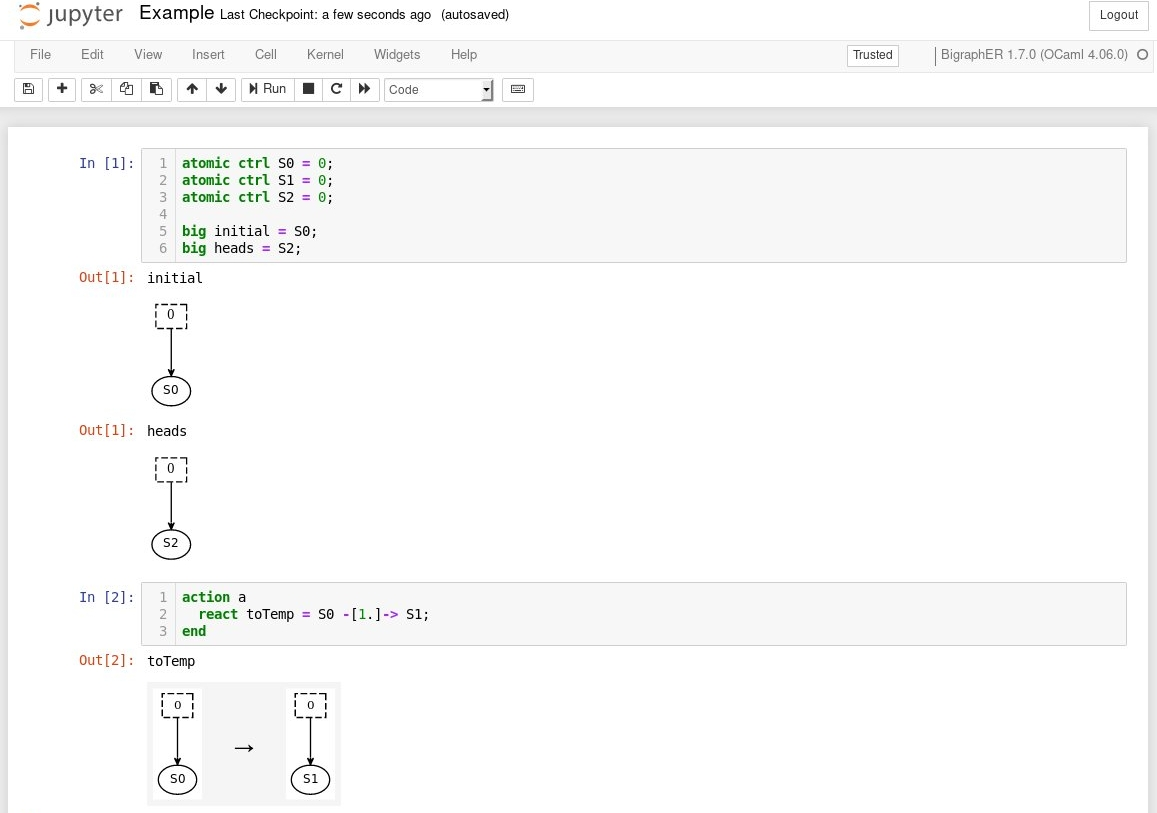
\includegraphics[width=\textwidth]{images/jupyter.jpg}
  \caption{The BigraphER Jupyter notebook interface with syntax highlighting.}
  \label{interface}
\end{figure}

We introduce a new front end to BigraphER based on Jupyter notebooks
\cite{DBLP:conf/elpub/KluyverRPGBFKHG16}. The BigraphER kernel is an extension
to the OCaml kernel\footnote{\url{https://github.com/akabe/ocaml-jupyter}} and
is available on
GitHub\footnote{\url{https://github.com/dilkas/bigrapher-jupyter}}. It supports
a similar workflow to that of Jupyter notebooks for other languages, allowing
the user to divide the code into multiple \emph{cells} and have the definitions
persist in a \emph{buffer} to be used later. By default, the output of each cell
displays the graphical representation of all bigraphs and reaction rules defined
in that cell (see Fig. \ref{interface} for an example). The generated images are
stored in a local directory \texttt{jupyter-images/}. The kernel also supports a
number of \emph{magics}, i.e., custom commands that can be used at the top of a
cell:

\begin{description}
  \item[\texttt{\%states}] produces a state transition diagram (similar to the
    one in Fig. \ref{example_ts}). Mousing over a state shows what that
    state looks like as a bigraph.
  \item[\texttt{\%simulate n}] runs a simulation for \texttt{n} steps, when used
    on non-stochastic models. For stochastic BRSs
    \cite{DBLP:journals/entcs/KrivineMT08}, \texttt{n} is interpreted as a
    floating-point number, representing maximum simulation time. The produced
    diagram is a single path through the transition system with the same
    mouse-over functionality.
  \item[\texttt{\%output}] displays the full output produced by BigraphER. By
    default, only errors are displayed in the notebook.
  \item[\texttt{\%ocaml}] allows full backward compatibility with the OCaml
    kernel, including auto-complete and integrated documentation features that
    have been extended to the BigraphER OCaml API as well as plotting support
    with Archimedes\footnote{\url{http://archimedes.forge.ocamlcore.org/}}.
  \item[\texttt{\%clear}] clears the buffer before interpreting the code from
    the current cell.
\end{description}

\section{A Case Study in Autonomous Agents}

In order to demonstrate the use of bigraphs in modelling probabilistic
processes with nondeterminism, we present two examples of agent movement
planning in two dimensions. The examples have different sources of probabilistic
behaviour and explore topics such as tracking visited locations and uncertainty
about the topology.

% TODO advantages: more visual/realistic than a vector of numbers, rewards and
% transition rules can be generated with a higher degree of automation, less
% code, more flexible (changing size of the grid); disadvantages: constant
% probability (without hacking)

% TODO xavier \cite{koenig1998xavier}

\subsection{Collecting Objects in a Grid}

Our first scenario is concerned with collecting objects in a grid-like
two-dimensional world and is inspired by similar scenarios modelled using PRISM
\cite{dblp:conf/nfm/giaquintahimn18,DBLP:conf/spin/HoffmannIMNV16}. The agent
starts in the southwest corner of the map (which we call \emph{home}), explores
the environment until it collects a specified number of objects, and returns
home (while possibly collecting more objects along the way). The model tracks
which cells of the grid have been explored, and only the unexplored cells have a
constant probability $p$ of rewarding the agent with an object. The desired
number of objects can be easily changed, and the map can be customised to make
some transitions unavailable (i.e. add walls), as long as the agent can still
return home.

\lstinputlisting[caption=Controls., captionpos=b, language=Big,
label=agent1_controls, firstline=3, lastline=14]{models/agent1.big}

We begin with a list of controls in Listing~\ref{agent1_controls}. On the right
hand side of each equal sign is the number of ports that each node of that
control has, while the \texttt{\textbf{atomic}} keyword specifies the nodes that
cannot contain other nodes. \texttt{Cell}s represents discrete locations. They
are linked to either \texttt{Visited} or \texttt{Unvisited} (initially, all
except one cells are unvisited). \texttt{Cell}s always contain
\texttt{Directions}, and one \texttt{Cell} contains an \texttt{Agent}. The
\texttt{Agent} may contain an \texttt{Object}. In order to represent multiple
objects, it is convenient to put the second \texttt{Object} inside the first,
and so on. \texttt{Directions} contains a subset of the four nodes,
corresponding to the four possible directions of travel: \texttt{North},
\texttt{East}, \texttt{West}, \texttt{South}. We connect neighbouring
\texttt{Cell}s by linking the \texttt{West} node of one \texttt{Cell} to the
\texttt{East} node of another (or \texttt{North} to \texttt{South}).

\lstinputlisting[caption=Predicates and the initial state., captionpos=b,
language=Big, label=agent1_code, firstline=16,
lastline=30]{models/agent1.big}

Next, we define two predicates: \texttt{home} and \texttt{goal} (see
Listing~\ref{agent1_code}). The former states that the agent is home if it is in
the southwest corner of the grid, while the latter specifies a goal of
collecting one object. A larger number of objects can be set by nesting
\texttt{Object}s inside each other, e.g., \texttt{Agent.Object.Object}.
Additionally, Listing~\ref{agent1_code} defines the initial $2 \times 2$ grid,
as described previously.

\lstinputlisting[caption=The action of going north., captionpos=b,
language=Big, label=agent1_north, firstline=88,
lastline=117]{models/agent1.big}

Then, we have an action for each of the four directions, each with three
reaction rules: one for going to an already visited cell, one for visiting a
cell for the first time, and one for visiting a cell for the first time and
finding an object. We will use the rules for going north in
Listing~\ref{agent1_north} as an example. When going to an already visited cell,
the \texttt{Agent} simply traverses a link between the \texttt{North} node of
its previous \texttt{Cell} and the corresponding \texttt{South} node. As this is
the only reaction rule for this situation, its probability is $1$. When going to
an unvisited node, we collect an \texttt{Object} with probability $p$, or make
the transition without getting an \texttt{Object} with probability $1-p$.
Regardless, the \texttt{Cell} changes its link from \texttt{Unvisited} to
\texttt{Visited}.

\lstinputlisting[caption=Reaction rule to stay home if a required number of
objects is acquired., captionpos=b, language=Big, label=agent1_home,
firstline=186, lastline=189]{models/agent1.big}

Lastly, we have three actions for when the agent acquires the specified number
of objects: two for going home west or south (since these are the two directions
necessary and sufficient to reach home), and one for staying home. The two
actions for going home have two reaction rules each, depending on whether the
destination cell is visited or not. They are just like the rules in
Listing~\ref{agent1_north}, except every mention of \texttt{Agent} is replaced
with \texttt{goal}. The rule to stay home simply says that if the agent has
achieved the goal, and is home (characterised by a \texttt{Cell} with only two
directions: \texttt{North} and \texttt{East}), then nothing should change (see
Listing~\ref{agent1_home}). To make the agent start heading home as soon as
enough objects are collected, all five reaction rules related to going and
staying home are in a higher priority class.

\subsection{Layers of Abstraction}

Our second model explores two important concepts in modelling the topology of
space: nesting and uncertainty. Nesting is the idea that spaces can be inside
other spaces: rooms inside floors, floors inside buildings, buildings inside
streets, etc. A key characteristic of nested spaces is that there is a separate
action (or several) taking you from the outer space to the inner space or vice
versa (e.g., using a door to enter or leave a room). In the rest of the paper,
whenever we discuss one space nested inside another, we will refer to the inner
space as the \emph{room}. While nesting has been modelled using bigraphs before
\cite{DBLP:conf/giscience/WaltonW12}, our approach models each room not as a
single entity, but rather as an interconnected collection of smaller spaces,
which we continue to call \emph{cells}. Thus, it is not enough to be in the
hallway in order to enter a room, one needs to be next to the door. Similarly,
after entering a room, the agent is positioned next to the other side of the
door.

The other concept explored in this section is uncertainty about the topology
itself, i.e., is the door open or closed? The implementation of this idea is
tied to that of rooms: the inside of a room is not defined until the outer cell
encompassing the room (i.e., the area where the door is located) is entered.
Then, the contents of the room are chosen from a finite set of possibilities
with a set probability distribution. After that, the room stays fixed. This
design decision supports the reality of missions with a reasonably short
duration: if the agent finds a locked door, it should not keep revisiting the
door hoping for it to suddenly be open.

As the ideas of collecting objects and tracking visited cells have been
explored already, they are dropped from this model in order to simplify the
implementation. The goal can simply be defined as moving from one location to
another. We add one extra control, \texttt{Node}. While \texttt{Cell} can be
imagined as a discrete patch of space (e.g., \SI{1}{\square\metre}),
\texttt{Node} can be thought of as a room. While we stick to two layers
(corridors and rooms) in this example, rooms can be freely nested: a room can
contain any number of rooms, each of which can contain more rooms.

\begin{figure}
  \centering
  \includegraphics{models/agent2/nesting_example/example.pdf}
  \caption{The bigraphical structure behind nesting.}
  \label{agent2_nesting}
\end{figure}

\lstinputlisting[caption={The initial map: three consecutive cells, the midmost
of which has an inner room.}, captionpos=b, language=Big, label=agent2_initial,
firstline=15, lastline=19]{models/agent2/agent.big}

\begin{figure}
  \centering
  \begin{minipage}{0.45\textwidth}
    \centering
    \includegraphics[width=\textwidth]{models/agent2/goIn_lhs.pdf}
  \end{minipage}
  $\longrightdoublearrowRHD$
  \begin{minipage}{0.45\textwidth}
    \centering
    \includegraphics[width=\textwidth]{models/agent2/goIn_rhs.pdf}
  \end{minipage}
  \caption{Left to right: the reaction rule to go inside; right to left: the
    reaction rule to go outside.}
  \label{go_in_out}
\end{figure}

In order to implement nesting, we put a \texttt{Node} (representing a room)
inside a \texttt{Cell}, which has the ``door'' to that room (see Fig.
\ref{agent2_nesting}). The \texttt{Node} can have its own collection of
\texttt{Cell}s, describing the topology of the room. One of these \texttt{Cell}s
is linked to the \texttt{Node}, representing the \texttt{Cell} closest to the
door from the inside of the room. Thus, both \texttt{Node}s and \texttt{Cell}s
have arity $1$ for exactly this linking. \texttt{Cell} ports not linked to
anything are implemented using closures (e.g. \texttt{/x Cell\{x\}}). The
initial map in Listing~\ref{agent2_initial} has a corridor of three cells with
the agent on the west-most cell and a door to a room in the middle cell. One
moves in and out of a room using a pair of actions with reaction rules pictured
in Fig.~\ref{go_in_out}.

\lstinputlisting[caption={Two ways to generate a room, leaving one door either
open or closed.}, captionpos=b, language=Big, label=agent2_room,
firstline=21, lastline=48]{models/agent2/agent.big}

\lstinputlisting[caption={The action of going north.}, captionpos=b,
language=Big, label=agent2_north, firstline=66,
lastline=75]{models/agent2/agent.big}

The room is a $2 \times 2$ grid of \texttt{Cell}s, which is generated when the
\texttt{Agent} gets to a \texttt{Cell} with an empty \texttt{Node} (represented
by \texttt{Node\{n\}.1})\footnote{Multiple different rooms can be implemented by
having each previously empty \texttt{Node} contain a node of different control.
This way a different probability distribution (with different possible outcomes)
can be assigned to each room.}. In order for the room to be generated before any
other action can take place, the two reaction rules in Listing~\ref{agent2_room}
are put on a higher priority class. With probability $p$, the generated room has
each \texttt{Cell} linked to its two neighbours; and with probability $1-p$, the
top two \texttt{Cell}s are not linked, possibly forcing the agent to choose a
different path. Finally, we have four actions, each with a single reaction rule
with probability $1$, corresponding to the four possible directions of travel.
The reaction rules are very similar to those of our previous example, an example
of which can be found in Listing~\ref{agent2_north}.

\section{Conclusion}

BIG TODO!

\bibliographystyle{splncs04}
\bibliography{bibliography}
\end{document}
